\documentclass[aspectratio=169]{beamer}
\usepackage[utf8]{inputenc}
\usepackage[T1]{fontenc}
\usepackage[brazil]{babel}
\usepackage{ragged2e}
\usepackage{booktabs}
\usepackage{verbatim}
\usetheme{AnnArbor}
\usecolortheme{orchid}
\usefonttheme[onlymath]{serif}
\usepackage{listings}

\lstset{language=C,
	backgroundcolor=\color{green!10},
	basicstyle=\ttfamily,
	keywordstyle=\color{blue}\ttfamily,
	stringstyle=\color{red}\ttfamily,
	commentstyle=\color{brown}\ttfamily,
	morecomment=[l][\color{magenta}]{\#}
}

\AtBeginSection[]{
  \begin{frame}
  \vfill
  \centering
  \begin{beamercolorbox}[sep=8pt,center,shadow=true,rounded=true]{title}
    \usebeamerfont{title}\insertsectionhead\par%
  \end{beamercolorbox}
  \vfill
  \end{frame}
}

\title[\sc{Recursão}]{Recursão}
\author[Roland Teodorowitsch]{Roland Teodorowitsch}
\institute[ALEST I - EP - PUCRS]{Algoritmos e Estruturas de Dados I - Escola Politécnica - PUCRS}
\date{14 de março de 2024}

\begin{document}
\justifying

%-------------------------------------------------------
\begin{frame}
	\titlepage
\end{frame}

%=======================================================
\section{Recursão}

%-------------------------------------------------------
\begin{frame}\frametitle{Leitura(s) Recomendada(s)}

\begin{columns}[T]
\begin{column}{0.15\linewidth}
\vspace{-3mm}
\begin{figure}[h]
	\centering
	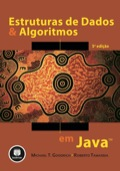
\includegraphics[height=0.3\paperheight]{imagens/livro_goodrich.jpg}
\end{figure}
\end{column}
\begin{column}{0.85\linewidth}
\vspace{3mm}
\textbf{Seção 3.5}\\
\scriptsize{GOODRICH, Michael T.; TAMASSIA, Roberto. \textbf{Estruturas de dados e algoritmos em Java}. Tradução: Bernardo Copstein. 5. ed. Porto Alegre: Bookman, 2013. xxii, 713 p. E-book. ISBN 9788582600191. Tradução de: Data Structures and Algorithms in Java, 5th Edition. Disponível em: \textless{}\url{https://integrada.minhabiblioteca.com.br/\#/books/9788582600191/}\textgreater{}. Acesso em: 01 ago. 2023.}
\end{column}
\end{columns}

\end{frame}

%-------------------------------------------------------
\begin{frame}\frametitle{Algoritmo Recursivo}
\begin{itemize}
	\item É um algoritmo que chamada a si próprio
	\item \textbf{Importante:} o algoritmo deve garantir que a recursão termine
	\begin{itemize}
		\item Caso contrário cria-se um ``laço infinito'' que causará um estouro de pilha
		\lstinputlisting{src/loop.cpp}
		\item Geralmente coloca-se uma condição de parada (situação em que a chamada recursiva NÃO é realizada) no início da implementação
	\end{itemize}
\end{itemize}
\end{frame}

%-------------------------------------------------------
\begin{frame}\frametitle{Exemplo clássico: Fatorial}
\begin{itemize}
	\item O fatorial de n é normalmente definido como:
\[ n! = \prod_{k=1}^{n}{k} = n \times (n-1) \times (n-2) \times ... \times 3 \times 2 \times 1,\qquad \forall n \in \mathbb{N}\]
	\item Por exemplo:
\[5 ! = 5 \times 4 \times 3 \times 2 \times 1 = 120\]
	\item Mas também pode-se usar a sua definição recursiva:
\[ n! = \begin{cases}
1, & \mbox{se ~ } n=0 \mbox{~ ou ~ } n=1\\
n \times (n-1)!, & \mbox{se ~ } n > 1
\end{cases} \]
\end{itemize}
\end{frame}

%-------------------------------------------------------
\begin{frame}[fragile]\frametitle{Implementação do Fatorial}
\begin{itemize}
	\item Iterativo
{\scriptsize\lstinputlisting{src/fatorial.cpp}}
	\item Recursivo
{\scriptsize\lstinputlisting{src/fatorialRec.cpp}}
\end{itemize}
\end{frame}

%-------------------------------------------------------
\begin{frame}\frametitle{Rastreamento Recursivo}
\begin{figure}[h]
	\centering
	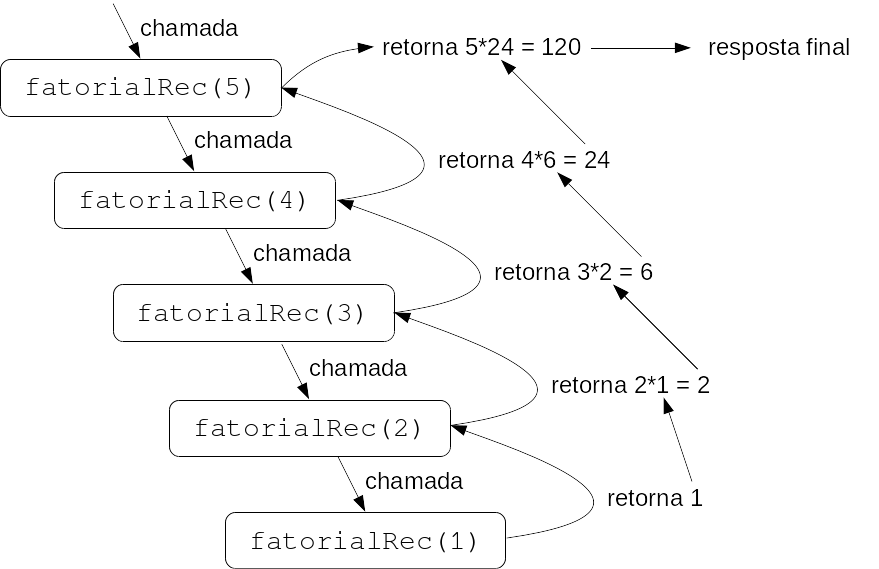
\includegraphics[height=0.7\paperheight]{imagens/rastreamento_recursivo.png}
\end{figure}
\end{frame}

%-------------------------------------------------------
\begin{frame}\frametitle{Exemplo: Contagem}
\begin{itemize}
	\item Iterativo
{\scriptsize\lstinputlisting{src/contagem.cpp}}
	\pause
	\item Recursivo
{\scriptsize\lstinputlisting{src/contagemRec.cpp}}
\end{itemize}
\end{frame}

%-------------------------------------------------------
\begin{frame}\frametitle{Exercício: Contagem Regressiva}
\begin{itemize}
	\item Iterativo
{\scriptsize\lstinputlisting{src/contagemRegressiva.cpp}}
	\pause
	\item Recursivo
{\scriptsize\lstinputlisting{src/contagemRegressivaRec.cpp}}
\end{itemize}
\end{frame}

%-------------------------------------------------------
\begin{frame}\frametitle{Exercício: Geração de Índices de uma Matriz}
\begin{itemize}
	\item Iterativo
{\scriptsize\lstinputlisting{src/indicesMatriz.cpp}}
	\pause
	\item Recursivo
{\scriptsize\lstinputlisting{src/indicesMatrizRec1.cpp}}
	\pause
	\item \textbf{Desafio:} faça uma versão recursiva do algoritmo acima sem usar nenhum laço!
\end{itemize}
\end{frame}

%-------------------------------------------------------
\begin{frame}\frametitle{Recursividade [*]}
\begin{itemize}
	\item Poderosa ferramenta de programação
	\item Apesar de bastante empregada, nem sempre ela deve ser aplicada
	\begin{itemize}
		\item É preciso analisar o problema e ver se necessita de uma solução recursiva
	\end{itemize}
	\item Quando bem empregada pode tornar a solução de um problema clara, simples e consisa
\end{itemize}
\end{frame}

%-------------------------------------------------------
\begin{frame}\frametitle{Vantagens [*]}
\begin{itemize}
	\item Rotinas mais concisas
	\item Relação direta com uma prova por indução matemática
	\begin{itemize}
		\item Indução matemática: metodo de prova matemática usado para demonstrar a verdade de um número infinito de proposições
		\begin{itemize}
			\item Válida se funciona para $n$ igual a $0$ ou $1$
			\item Válida se vale para $n$ igual a $k$ e $k + 1$
		\end{itemize}
		\item Facilita verificar a correção
	\end{itemize}
\end{itemize}
\end{frame}

%-------------------------------------------------------
\begin{frame}\frametitle{Desvantagens [*]}
\begin{itemize}
	\item Cada chamada recursiva implica em um custo (tempo e espaço)
	\begin{itemize}
		\item Informações são armazenadas na pilha
		\item Para cada chamada realizada, um conjunto de variáveis locais é alocado (criado)
		\item Cada chamada requer
		\begin{itemize}
			\item O empilhamento de parâmetros e endereços de retorno da função que chama
			\item A alocação de variáveis locais da função % [Roland]
			%\item O desempilhamento de parâmetros pela função que executa
		\end{itemize}
		\item Cada retorno requer
		\begin{itemize}
			\item A desalocação das variáveis locais da função % [Roland]
			\item O desempilhamento do endereço de retorno
			%\item O empilhamento do resultado (ou passagem por registrador)
			%\item O desempilhamento do retorno pela função que chamou
		\end{itemize}
	\end{itemize}
\end{itemize}
\end{frame}

%=======================================================
\section{Algoritmos de Pesquisa}

%-------------------------------------------------------
\begin{frame}\frametitle{Algoritmos de Pesquisa}
\begin{itemize}
	\item Localizam um elemento dentro de uma coleção
	\item Podem retornar
	\begin{itemize}
		\item \textbf{Valor booleano} (\texttt{true} se o elemento existir na coleção ou \texttt{false}, em caso contrário) ou
		\item \textbf{Índice} (posição) do elemento na coleção (ou -1 se não encontrar)
	\end{itemize}
	\item Para coleções \textbf{desordenadas}, deve-se usar um algoritmo de \textbf{pesquisa linear}
	\item Quando a coleção está \textbf{ordenada}, pode-se usar um algoritmo de \textbf{pesquisa binária}
\end{itemize}
\end{frame}

%-------------------------------------------------------
\begin{frame}\frametitle{Pesquisa Linear}
\begin{itemize}
	\item Serve para coleções \textbf{desordenadas}
	\item Estratégia: comparar o elemento procurado com cada item da coleção até encontrar ou até chegar ao fim
	\item Melhor caso: o elemento procurado é o primeiro da lista
	\item Pior caso: o elemento procurado \textbf{NÃO} existe na lista
	\item Também poderia ser aplicado sobre coleções ordenadas
	\pause
	\item Complexidade: $O(n)$
\end{itemize}
\end{frame}

%-------------------------------------------------------
\begin{frame}[fragile]\frametitle{Implementação da Pesquisa Linear}
\begin{itemize}
	\item Iterativo
{\scriptsize\lstinputlisting{src/pesquisaLinear.cpp}}
	\pause
	\item Recursivo
{\scriptsize\lstinputlisting{src/pesquisaLinearRec.cpp}}
\end{itemize}
\end{frame}

%-------------------------------------------------------
\begin{frame}\frametitle{Pesquisa Binária}
\begin{itemize}
	\item Serve \textbf{APENAS} para coleções \textbf{ordenadas}
	\item Estratégia:
	\begin{itemize}
		\item Compara o valor procurado com o elemento do meio
		\begin{itemize}
			\item Se for igual, encontrou
			\item Se for menor, continua-se a busca na metade inferior (desconsidera a metade superior)
			\item Se for maior, continua-se a busca na metade superior (desconsidera a metade inferior)
		\end{itemize}
		\item Repete-se o procecimento até que o valor procurado seja encontrado ou até que não se consiga dividir a coleção
	\end{itemize}
	\pause
		\item Complexidade: $O(\log{n})$
\end{itemize}
\end{frame}

%-------------------------------------------------------
\begin{frame}[fragile]\frametitle{Pesquisa Binária Iterativa}
\lstinputlisting[basicstyle=\ttfamily\scriptsize]{src/pesquisaBinaria.cpp}
\end{frame}

%-------------------------------------------------------
\begin{frame}\frametitle{Pesquisa Binária: Exemplo (\texttt{valor = 18})}
\begin{itemize}

	\item Passo 1:
\begin{tabular}{cccccccccc}
\tiny{0} & \tiny{1} & \tiny{2} & \tiny{3} & \tiny{4} & \tiny{5} & \tiny{6} & \tiny{7} & \tiny{8} & \tiny{9}\\
\hline
\multicolumn{1}{|c|}{2} & \multicolumn{1}{c|}{4} & \multicolumn{1}{c|}{6} & \multicolumn{1}{c|}{8} & \multicolumn{1}{c|}{10} & \multicolumn{1}{c|}{12} & \multicolumn{1}{c|}{14} & \multicolumn{1}{c|}{16} & \multicolumn{1}{c|}{18} & \multicolumn{1}{c|}{20}\\
\hline
$\uparrow$ & & & & $\uparrow$ & & & & & $\uparrow$ \\
{\tiny\texttt ini} & & & & {\tiny\texttt meio} & & & & & {\tiny\texttt fim} \\
\end{tabular}

	\item Passo 2:
\begin{tabular}{cccccccccc}
\tiny{0} & \tiny{1} & \tiny{2} & \tiny{3} & \tiny{4} & \tiny{5} & \tiny{6} & \tiny{7} & \tiny{8} & \tiny{9}\\
\hline
\multicolumn{1}{|c|}{2} & \multicolumn{1}{c|}{4} & \multicolumn{1}{c|}{6} & \multicolumn{1}{c|}{8} & \multicolumn{1}{c|}{10} & \multicolumn{1}{c|}{12} & \multicolumn{1}{c|}{14} & \multicolumn{1}{c|}{16} & \multicolumn{1}{c|}{18} & \multicolumn{1}{c|}{20}\\
\hline
 & & & & & $\uparrow$ & & $\uparrow$ & & $\uparrow$ \\
 & & & & & {\tiny\texttt ini} & & {\tiny\texttt meio} & & {\tiny\texttt fim} \\
\end{tabular}

	\item Passo 3:
\begin{tabular}{cccccccccc}
\tiny{0} & \tiny{1} & \tiny{2} & \tiny{3} & \tiny{4} & \tiny{5} & \tiny{6} & \tiny{7} & \tiny{8} & \tiny{9}\\
\hline
\multicolumn{1}{|c|}{2} & \multicolumn{1}{c|}{4} & \multicolumn{1}{c|}{6} & \multicolumn{1}{c|}{8} & \multicolumn{1}{c|}{10} & \multicolumn{1}{c|}{12} & \multicolumn{1}{c|}{14} & \multicolumn{1}{c|}{16} & \multicolumn{1}{c|}{18} & \multicolumn{1}{c|}{20}\\
\hline
 & & & & & & & & $\uparrow$ & $\uparrow$ \\
 & & & & & & & & {\tiny\texttt ini} & {\tiny\texttt fim} \\
 & & & & & & & & {\tiny\texttt meio} & \\
\end{tabular}
 ~ Valor 18 encontrado no índice 8!
\end{itemize}
\end{frame}

%-------------------------------------------------------
\begin{frame}\frametitle{Pesquisa Binária: Exemplo (\texttt{valor = 5})}
\begin{itemize}

	\item Passo 1:
\begin{tabular}{cccccccccc}
\tiny{0} & \tiny{1} & \tiny{2} & \tiny{3} & \tiny{4} & \tiny{5} & \tiny{6} & \tiny{7} & \tiny{8} & \tiny{9}\\
\hline
\multicolumn{1}{|c|}{2} & \multicolumn{1}{c|}{4} & \multicolumn{1}{c|}{6} & \multicolumn{1}{c|}{8} & \multicolumn{1}{c|}{10} & \multicolumn{1}{c|}{12} & \multicolumn{1}{c|}{14} & \multicolumn{1}{c|}{16} & \multicolumn{1}{c|}{18} & \multicolumn{1}{c|}{20}\\
\hline
$\uparrow$ & & & & $\uparrow$ & & & & & $\uparrow$ \\
{\tiny\texttt ini} & & & & {\tiny\texttt meio} & & & & & {\tiny\texttt fim} \\
\end{tabular}\\~\\~

	\item Passo 2:
\begin{tabular}{cccccccccc}
\tiny{0} & \tiny{1} & \tiny{2} & \tiny{3} & \tiny{4} & \tiny{5} & \tiny{6} & \tiny{7} & \tiny{8} & \tiny{9}\\
\hline
\multicolumn{1}{|c|}{2} & \multicolumn{1}{c|}{4} & \multicolumn{1}{c|}{6} & \multicolumn{1}{c|}{8} & \multicolumn{1}{c|}{10} & \multicolumn{1}{c|}{12} & \multicolumn{1}{c|}{14} & \multicolumn{1}{c|}{16} & \multicolumn{1}{c|}{18} & \multicolumn{1}{c|}{20}\\
\hline
$\uparrow$ & $\uparrow$ & & $\uparrow$ & & & & & & \\
{\tiny\texttt ini} & {\tiny\texttt meio}& & {\tiny\texttt fim} & & & & & & \\
\end{tabular}

\end{itemize}
\end{frame}

%-------------------------------------------------------
\begin{frame}\frametitle{Pesquisa Binária: Exemplo (\texttt{valor = 5})}
\begin{itemize}

	\item Passo 3:
\begin{tabular}{cccccccccc}
\tiny{0} & \tiny{1} & \tiny{2} & \tiny{3} & \tiny{4} & \tiny{5} & \tiny{6} & \tiny{7} & \tiny{8} & \tiny{9}\\
\hline
\multicolumn{1}{|c|}{2} & \multicolumn{1}{c|}{4} & \multicolumn{1}{c|}{6} & \multicolumn{1}{c|}{8} & \multicolumn{1}{c|}{10} & \multicolumn{1}{c|}{12} & \multicolumn{1}{c|}{14} & \multicolumn{1}{c|}{16} & \multicolumn{1}{c|}{18} & \multicolumn{1}{c|}{20}\\
\hline
 & & $\uparrow$ & $\uparrow$ & & & & & & \\
 & & {\tiny\texttt ini} & {\tiny\texttt fim} & & & & & & \\
 & & {\tiny\texttt meio} & & & & & & & \\
\end{tabular}\\~\\~

	\item Passo 4:
\begin{tabular}{cccccccccc}
\tiny{0} & \tiny{1} & \tiny{2} & \tiny{3} & \tiny{4} & \tiny{5} & \tiny{6} & \tiny{7} & \tiny{8} & \tiny{9}\\
\hline
\multicolumn{1}{|c|}{2} & \multicolumn{1}{c|}{4} & \multicolumn{1}{c|}{6} & \multicolumn{1}{c|}{8} & \multicolumn{1}{c|}{10} & \multicolumn{1}{c|}{12} & \multicolumn{1}{c|}{14} & \multicolumn{1}{c|}{16} & \multicolumn{1}{c|}{18} & \multicolumn{1}{c|}{20}\\
\hline
 & $\uparrow$ & $\uparrow$ & & & & & & & \\
 & {\tiny\texttt fim} & {\tiny\texttt ini} & & & & & & & \\
\end{tabular}
 ~ Valor 5 \textbf{NÃO} encontrado!

\end{itemize}
\end{frame}

%-------------------------------------------------------
\begin{frame}[fragile]\frametitle{Pesquisa Binária Recursiva}
\lstinputlisting[basicstyle=\ttfamily\scriptsize]{src/pesquisaBinariaRec.cpp}
\end{frame}

%=======================================================
\section{Exercícios}

%-------------------------------------------------------
\begin{frame}\frametitle{Exercícios}
\begin{enumerate}
	\item Dado um valor inteiro e positivo (\texttt{n}), o valor da constante de \emph{Euler} poder ser calculando com precisão diretamente proporcional a \texttt{n} através da fórmula:
\[ E = \frac{1}{0!} + \frac{1}{1!} + \frac{1}{2!}+ \frac{1}{3!} + ... + \frac{1}{n!}\]
Implemente, em C, um método recursivo que recebe \texttt{n}, retornando o valor de \emph{Euler} calculado usando a fórmula acima.
	\item Considere a função abaixo, que implementa o somatório de um vetor e implemente a sua versão recursiva.
\lstinputlisting[basicstyle=\ttfamily\tiny]{src/somatorio.cpp}
\end{enumerate}
\end{frame}

%-------------------------------------------------------
\begin{frame}\frametitle{Exercícios}
\begin{enumerate}
        \setcounter{enumi}{2}
	\item Considere a função que implementa o algoritmo \emph{Bubble Sort} (apresentada na unidade anterior) e implemente a sua versão recursiva).
	\item Implemente uma função recursiva que inverte os elementos de um vetor, trocando o primeiro elemento com o último, o segundo com o penúltimo, e assim sucessivamente.
	\item Implemente uma função recursiva que verifica se uma cadeia de caracteres recebida como parâmetro é um palíndromo ou não. Por exemplo, ``socorrammesubinoonibusemmarrocos'' é um palíndromo.
	%\item Faça o algoritmo da potência de forma não recursiva e de forma recursiva. Considere que o valor da base e do expoente são recebidos por parâmetro, inteiros e positivos.
\end{enumerate}
\end{frame}

%=======================================================
\section{Créditos}

%-------------------------------------------------------
\begin{frame}\frametitle{Créditos}
\begin{itemize}
	\item Estas lâminas contêm trechos adaptados de materiais criados e disponibilizados pelo professor Iaçanã Ianiski Weber [*].
\end{itemize}
\end{frame}

%=======================================================
\section{Soluções}

%-------------------------------------------------------
\begin{frame}\frametitle{Soluções}
\begin{enumerate}
	\item \lstinputlisting[basicstyle=\ttfamily\tiny]{src/eulerRec.cpp}

	\item \lstinputlisting[basicstyle=\ttfamily\tiny]{src/somatorioRec.cpp}

	\item \lstinputlisting[basicstyle=\ttfamily\tiny]{src/bubbleSortRec.cpp}
\end{enumerate}
\end{frame}

%-------------------------------------------------------
\begin{frame}\frametitle{Soluções}
\begin{enumerate}
        \setcounter{enumi}{3}
	\item \lstinputlisting[basicstyle=\ttfamily\tiny]{src/inverteVetorRec.cpp}

	\item \lstinputlisting[basicstyle=\ttfamily\tiny]{src/palindromoRec.cpp}

\end{enumerate}
\end{frame}

%-------------------------------------------------------
\end{document}

